\documentclass[11pt,a4paper]{article}

\usepackage[T2A]{fontenc}
\usepackage[utf8]{inputenc}
\usepackage[english,russian]{babel}

\usepackage[a4paper, 
            lmargin=0.1666\paperwidth, 
            rmargin=0.1666\paperwidth, 
            tmargin=0.1111\paperheight, 
            bmargin=0.1111\paperheight]{geometry}

\usepackage{mathptmx}
\usepackage{amsmath}
\usepackage{amssymb}

\usepackage{graphicx}
\usepackage{float}

\title{Аналитическое и численное решение задачи методом наименьших квадратов}
\author{Евгений Баяк}
\date{Октябрь 2024}

\begin{document}

\maketitle

\section*{Введение}
Метод наименьших квадратов -- это фундаментальный статистический метод, широко используемый в машинном обучении для регрессионного анализа. Он направлен на поиск наиболее подходящей линии или кривой для заданного набора данных путем минимизации суммы квадратов остатков (разниц между наблюдаемыми и прогнозируемыми значениями).

\section{Аналитическое решение}

\subsection{Общий случай}
Имеется набор из $n$ значений переменной $y$ (например, результаты наблюдений или экспериментов) и соответствующие им переменные $x$. Задача состоит в том, чтобы аппроксимировать зависимость между $y$ и $x$ с помощью некоторой функции $f(x, b)$, которая зависит от неизвестных параметров $b$. Необходимо найти такие значения параметров $b$, которые наилучшим образом соответствуют предсказанным значениям $f(x, b)$ реальным значениям $y$. Это можно рассматривать как задачу «решения» переопределенной системы уравнений для параметров $b$:

\begin{equation}
f(x_t,b)=y_t, \quad t=1, \ldots, n.
\end{equation}

В регрессионном анализе и в частности в эконометрике используются вероятностные модели зависимости между переменными

\begin{equation}
y_t=f(x_t,b)+\varepsilon_t,
\end{equation}

где $\varepsilon_t$~-- случайные ошибки модели.

Соответственно, отклонения наблюдаемых значений $y$ от модельных $f(x,b)$ уже учитываются в самой модели. Оценка параметров $\hat b_{OLS}$ (OLS, от английского Ordinary Least Squares), при которых сумма квадратов отклонений $e_t$ достигает минимального значения выражается формулой:

\begin{equation}
\hat b_{OLS}=\arg \min_{b}RSS(b),
\end{equation}

где $RSS$~-- Residual Sum of Squares~-- это мера, используемая в регрессионном анализе для оценки качества модели. Она определяется как сумма квадратов остатков, то есть разностей между наблюдаемыми значениями и предсказанными значениями модели и определяется как:

\begin{equation} \label{eq:4}
RSS(b)=e^Te=\sum_{t=1}^n e^2_t=\sum_{t=1}^n (y_t-f(x_t,b))^2.
\end{equation}

Чтобы минимизировать $RSS$ по параметрам $b$, необходимо продифференцировать его по $b$ и приравнять к нулю. Аналитическое решение задачи, основанное на методе наименьших квадратов, в общем случае выражается уравнением~\cite{magnus}:

\begin{equation} \label{eq:5}
\sum_{t=1}^n(y_t-f(x_t,b))\frac {\partial f(x_t,b)}{\partial b}=0 .
\end{equation}

\subsection{Линейная регрессия}
Пусть задана обучающая выборка $S = \left\{ (\bar{x}_1, y_1), \ldots, (\bar{x}_l, y_l) \right\}$, где $\bar{x}_i \in \mathbb{R}^n$ и $y_i \in \mathbb{R}$ для $i = 1, \ldots, l$. Задача линейной регрессии заключается в нахождении линейной функции:

\begin{equation}
f(\bar{x}) = (\bar{w} \cdot \bar{x}) + b,
\end{equation}

которая наилучшим образом интерполирует элементы выборки $S$. Геометрически данная функция представляет собой гиперплоскость, которая приближает точки $y_i$ на аргументах $x_i$ при $i = 1, \ldots, l$.

Данная задача была решена Гауссом и Лежандром еще в XVIII веке при помощи минимизации суммы квадратов разностей значений функции $f(\bar{x}_i)$ и точек $y_i$ при $i = 1, \ldots, l$. Теория обобщения для данного метода хорошо представлена в математической статистике для случая линейной модели генерации данных с гауссовским случайным шумом.

\subsection{Метод наименьших квадратов}
Функция потерь $L$ для модели линейной регрессии определена как сумма квадратов разностей между наблюдаемыми значениями $y_i$ и прогнозируемыми значениями $f(\bar{x}_i)$:

\begin{equation}
L(\bar{w}, b) = \sum_{i=1}^{n} (y_i - f(\bar{x}_i))^2 = \sum_{i=1}^{n} (y_i - (\bar{w} \cdot \bar{x}_i + b))^2
\end{equation}

Задача метода наименьших квадратов~-- минимизировать функцию потерь $L$.

Пусть $\tilde{w}$ -- расширенный вектор-столбец весовых коэффициентов и свободного члена:

\begin{equation}
\tilde{w} = 
\begin{pmatrix}
w_1 \\
w_2 \\
\vdots \\
w_n \\
b
\end{pmatrix}
\end{equation}

Аналогичным образом, $\tilde{x}$ -- расширенный вектор-столбец переменных:

\begin{equation}
\tilde{x} = 
\begin{pmatrix}
x_1 \\
x_2 \\
\vdots \\
x_n \\
1
\end{pmatrix}
\end{equation}

В новых расширенных переменных функция регрессии имеет однородный вид без свободного члена:

\begin{equation}
f(\tilde{x}) = (\tilde{w} \cdot \tilde{x}).
\end{equation}

Тогда матрица типа $(l \times (n + 1))$, строками которой являются расширенные векторы-строки $\tilde{x}_i' = (\bar{x}_i', 1)$ переменных обозначается

\begin{equation}
\tilde{X} = 
\begin{pmatrix}
\tilde{x}_1' \\
\tilde{x}_2' \\
\vdots \\
\tilde{x}_l'
\end{pmatrix}
=
\begin{pmatrix}
x_{11} &  \hdots & x_{1n} & 1 \\
x_{21} & \hdots & x_{2n} & 1 \\ 
\vdots & \ddots & \vdots & \vdots \\
x_{l1} & \hdots & x_{ln} & 1
\end{pmatrix}.
\end{equation}

Также введен $l$-мерный вектор-столбец значений интерполяции

\begin{equation}
\hat{y} = 
\begin{pmatrix}
y_1 \\
y_2 \\
\vdots \\
y_l
\end{pmatrix}.
\end{equation}

Разности $|f(\bar{x}_i) - y_i|$ называются остатками. Вектор-столбец остатков имеет вид $\bar{y} - (\tilde{X} \tilde{\bar{w}})$, а функционал можно записать в матричном виде как квадрат нормы вектора-столбца остатков:

\begin{equation}
L(\tilde{w}) = \|\tilde{X} \tilde{w} - y\|^2 = (y - \tilde{X} \tilde{w})' (y - \tilde{X} \tilde{w}).
\end{equation}

Теперь задача регрессии может быть записана в виде задачи минимизации квадрата нормы вектора остатков:

\begin{equation}
L(\tilde{w}) = \|\tilde{X} \tilde{w} - y\|^2 \rightarrow \min.
\end{equation}

\sloppy
Геометрически это может интерпретироваться как поиск проекции наименьшей длины вектора $\bar{y}$ на подпространство (гиперплоскость), порожденное векторами-столбцами матрицы $\tilde{X}$.

Для поиска минимума приравниваем частные производные этого функционала (по переменным $w_1, \ldots, w_n, b$) к нулю. Получим систему из $n + 1$ уравнений.

\begin{equation}
\frac{\partial L(\tilde{w})}{\partial \tilde{w}} = 2 \tilde{X}^T (\tilde{X} \tilde{w} - y)^T = \bar{0}.
\end{equation}

Cистема упрощается к виду:

\begin{equation}
\tilde{X}^T \tilde{X} \tilde{w} = \tilde{X}^T y.
\end{equation}

Если матрица $\tilde{X}^T \tilde{X}$ обратима, решение получается по формуле \cite{vyugin}:

\begin{equation}
\tilde{w} = (\tilde{X}^T \tilde{X})^{-1} \tilde{X}^T y.
\end{equation}

\section{Численное решение}

Численное решение задачи наименьших квадратов представляет собой важный аспект регрессионного анализа, позволяющий находить параметры модели, которые минимизируют сумму квадратов отклонений между наблюдаемыми и предсказанными значениями. В отличие от линейных моделей, где решение может быть найдено аналитически, в случае нелинейных моделей требуется применение численных методов.

Одним из наиболее распространенных методов для решения задач нелинейных наименьших квадратов является метод Гаусса-Ньютона. Этот метод основан на итеративном решении линейных задач наименьших квадратов, которые возникают при каждом шаге итерации. Основная идея заключается в том, чтобы линейно аппроксимировать функцию потерь в окрестности текущего приближения параметров и затем решать соответствующую линейную задачу.

Другим подходом является метод Левенберга-Маркардта, который сочетает в себе преимущества метода Гаусса-Ньютона и градиентного спуска. Этот метод адаптирует шаг итерации в зависимости от того, насколько хорошо текущая модель описывает данные, что позволяет более эффективно находить минимум функции потерь.

Для успешного применения методов нелинейных наименьших квадратов важно иметь начальные приближения для параметров, так как они могут существенно повлиять на сходимость алгоритма. Численные методы для решения задач нелинейных наименьших квадратов являются мощными инструментами в статистическом моделировании, позволяя эффективно находить параметры для сложных моделей.

\subsection{Метод Гаусса-Ньютона}
Метод Гаусса-Ньютона является одним из наиболее распространенных численных методов для решения задач нелинейных наименьших квадратов. Как уже упоминалось, задача заключается в минимизации суммы квадратов остатков по формуле \ref{eq:4}. Пусть вектор остатков $\mathbf{g}(b)$ определяется как:

\begin{equation}
\mathbf{g}(b) = \begin{bmatrix}
y_1 - f(x_1, b) \\
y_2 - f(x_2, b) \\
\vdots \\
y_n - f(x_n, b)
\end{bmatrix}.
\end{equation}

Метод предполагает, что функция $f(x, b)$ является дифференцируемой. Чтобы минимизировать $RSS$ по параметрам $b$, необходимо продифференцировать его по $b$ и приравнять к нулю. Для этого используется разложение Тейлора для вектора остатков $\mathbf{g}(\hat b+h)$ в окрестности текущего приближения $\hat b$:

\begin{equation}
\mathbf{g}(\hat b + h) \approx \mathbf{g}(\hat b) + J(\hat b) h,
\end{equation}

где матрица Якоби $J(\hat b)$ имеет размерность  $n \times k$ (при этом  $n \geq k$) и определяется как:

\begin{equation}
J(\hat b) = \begin{bmatrix}
\frac{\partial g_1}{\partial b_1}(b) & \frac{\partial g_1}{\partial b_2}(b) & \cdots & \frac{\partial g_1}{\partial b_k}(b) \\
\frac{\partial g_2}{\partial b_1}(b) & \frac{\partial g_2}{\partial b_2}(b) & \cdots & \frac{\partial g_2}{\partial b_k}(b) \\
\vdots & \vdots & \ddots & \vdots \\
\frac{\partial g_n}{\partial b_1}(b) & \frac{\partial g_n}{\partial b_2}(b) & \cdots & \frac{\partial g_n}{\partial b_k}(b)
\end{bmatrix}.
\end{equation}

Можно пренебречь остатком в разложении Тейлора. Подставляя разложение Тейлора в выражение для $RSS(b)$, получается:

\begin{equation}
RSS(\hat{b} + h) \approx L(h) = RSS(\hat b) + J(\hat b) h^T \mathbf{g}(\hat b) + \frac{1}{2} h^T J(\hat b)^T J(\hat b) h.
\end{equation}

Относительно $h$ для упрощения можно обозначить $J(\hat b) = J$ и $\mathbf{g}(\hat b) = \mathbf{g}$. Градиент функции \( L \):

\begin{equation}
L'(h) = J^T \mathbf{g} + J^T J h.
\end{equation}

Гессиан \( L''(h) = J^T J \) является независимым от \( h \) и симметричным. Если матрица Якоби \( J \) имеет полный ранг (то есть столбцы линейно независимы), то гессиан будет положительно определённым. Это означает, что функция \( L(h) \) имеет уникальный минимум.

Чтобы найти параметры $b$, минимизирующие $RSS$, необходимо решить уравнение:

\begin{equation}
(J^T J) h = -J^T \mathbf{g}.
\end{equation}

Этот шаг позволяет вычислить обновление параметров по формуле:

\begin{equation}
\hat b_{k+1} = \hat b_k - (J^T J)^{-1} J^T \mathbf{g}(\hat b_k).
\end{equation}

где $\mathbf{g}(\hat b_k)$ — вектор остатков, вычисленный на текущем шаге. Процесс повторяется до тех пор, пока изменения в параметрах не станут достаточно малыми, что указывает на сходимость алгоритма.

Метод Гаусса-Ньютона эффективен для задач, где функция $f(x, b)$ является гладкой и хорошо аппроксимируется линейной моделью в окрестности решения. Однако, как и любой итеративный метод, он требует хороших начальных приближений для параметров, чтобы обеспечить сходимость к глобальному минимуму \cite{madsen}.


\section{Реализация}

В Python можно реализовать метод наименьших квадратов используя библиотеки. Ниже приведен простой пример с использованием NumPy:

\begin{verbatim}
import numpy as np
import matplotlib.pyplot as plt

x = np.array([1, 2, 3, 4, 5])
y = np.array([2, 3, 5, 7, 11])

A = np.vstack([x, np.ones(len(x))]).T
m, c = np.linalg.lstsq(A, y, rcond=None)[0]

plt.plot(x, y, 'o', label='данные', markersize=10)
plt.plot(x, m*x + c, 'r', label=f'y = {m:.2f}x + {c:.2f}')
plt.legend()
plt.show()
\end{verbatim}

В этом коде показано, как с помощью метода наименьших квадратов подогнать линию к набору точек данных и визуализировать результаты. На рисунке \ref{fig:fig1} изображен график результата работы фрагмента кода. Полученная линия минимизирует сумму квадратов расстояний до точек.

\begin{figure}[H]
    \centering
    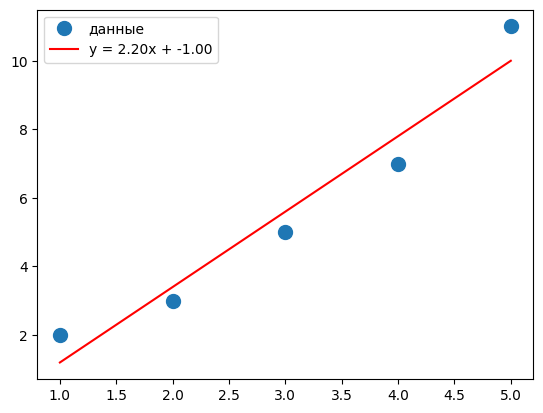
\includegraphics[width=0.75\linewidth]{OLS-example-np-lstsq.png}
    \caption{Линейная регрессия}
    \label{fig:fig1}
\end{figure}

Ниже приведен пример кода на Python, который реализует метод Гаусса-Ньютона для нахождения параметров экспоненциальной модели.

\begin{verbatim}
import numpy as np
import matplotlib.pyplot as plt

x_data = np.array([0, 1, 2, 3, 4])
y_data = np.array([1, 2.7, 7.4, 20.1, 54.6])

a = 1.0
b = 0.5

def residuals(params, x, y):
    a, b = params
    return y - a * np.exp(b * x)

for _ in range(20):
    r = residuals((a, b), x_data, y_data)
    J = np.column_stack(
        (-np.exp(b * x_data), -a * x_data * np.exp(b * x_data))
    )
    delta = np.linalg.inv(J.T @ J) @ J.T @ r
    a -= delta[0]
    b -= delta[1]

x = np.linspace(0, 4, 100)
y = a * np.exp(b * x)
plt.scatter(x_data, y_data, label='данные', color='blue')
plt.plot(x, y, color='red', label=f'y = {a:.2f}*e^({b:.2f}*x)')
plt.xlabel('x')
plt.ylabel('y')
plt.legend()
plt.show()
\end{verbatim}

Метод Гаусса-Ньютона используется для минимизации суммы квадратов отклонений между наблюдаемыми значениями и предсказанными значениями модели, заданной уравнением  
$y = a \cdot e^{b \cdot x}$ . 

В процессе работы кода сначала инициализируются параметры $a$  и  $b$, затем вычисляются остатки между фактическими и предсказанными значениями. Далее формируется матрица Якоби, которая используется для обновления параметров в каждой итерации. После нескольких итераций получаются оптимальные значения параметров, которые минимизируют отклонения.
На рисунке \ref{fig:fig2} отображаются исходные точки данных и полученная модель. Полученная кривая демонстрирует, как модель хорошо соответствует данным, минимизируя сумму квадратов расстояний до точек.

\begin{figure}[H]
    \centering
    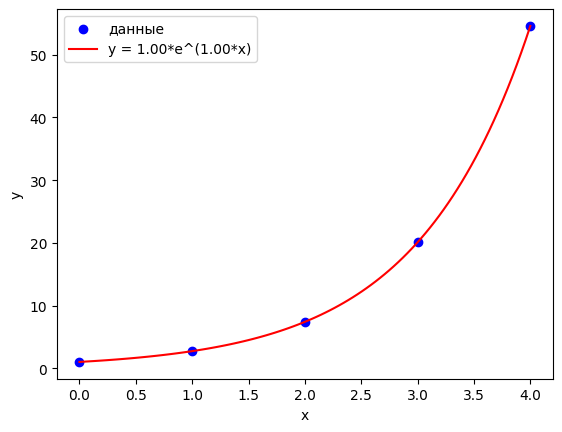
\includegraphics[width=0.75\linewidth]{gauss-newton-example.png}
    \caption{Нелинейная регрессия}
    \label{fig:fig2}
\end{figure}


\section*{Заключение}

Метод наименьших квадратов является мощным инструментом в области машинного обучения, предлагающим простой и эффективный подход к регрессионному анализу. Его основное предназначение заключается в минимизации суммы квадратов отклонений между наблюдаемыми и предсказанными значениями, что позволяет находить оптимальные параметры модели. Этот метод широко используется в различных областях, таких как экономика, физика и социология, где необходимо анализировать данные и делать прогнозы на основе исторической информации.

Преимуществом метода наименьших квадратов является его простота и интуитивная интерпретация, что позволяет выявлять зависимости между переменными. Он также служит основой для более сложных алгоритмов машинного обучения, таких как регрессионные деревья и нейронные сети.

Кроме того, метод легко реализуется с помощью различных программных библиотек, что делает его доступным для специалистов с разным уровнем подготовки. В условиях растущих объемов данных и потребности в точных прогнозах метод наименьших квадратов продолжает оставаться актуальным инструментом для анализа и обработки данных.


\begin{thebibliography}{9}
\bibitem{magnus}
Магнус, Я. Р. Катышев П.К., Пересецкий А.А. Эконометрика. Начальный курс: Учеб. / Я. Р. Магнус, П. К. Катышев, А. А. Пересецкий -- 6-е изд., перераб. и доп. -- М.: Дело, 2004. -- 576 с.

\bibitem{vyugin}
Вьюгин, В. В. Математические основы теории машинного обучения и прогнозирования / В.В. Вьюгин -- М.: 2013. -- 387 с.

\bibitem{madsen}
Madsen K. -- Methods for non-linear least squares problems / K.~Madsen, H.~B.~Nielsen, O. Tingleff. -- 2nd ed. -- Informatics and Mathematical Modelling, Technical University of Denmark~-- 2004~-- 58 p.
\end{thebibliography}

\end{document}
